\documentclass[../main.tex]{subfiles}
\usepackage{graphicx}
\usepackage{subcaption}
\usepackage{adjustbox}

\begin{document}

\begin{figure}[H]
    \begin{tabular}{c c}
        \begin{subfigure}{0.5\textwidth} 
            \centering
            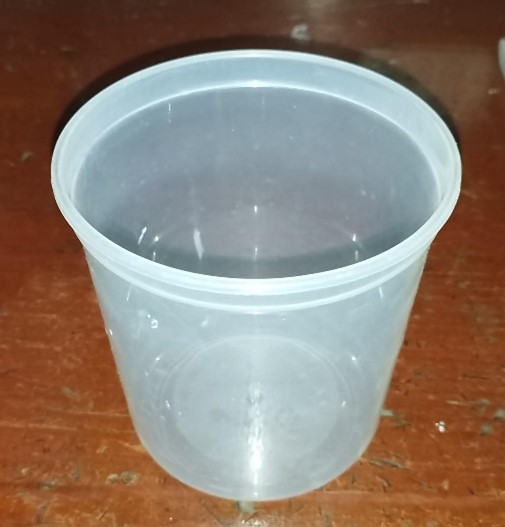
\includegraphics[width=0.8\linewidth,height=0.6\linewidth]{resources/mat1.jpg}
            \caption{Vaso}
            \label{fig:mat1}
        \end{subfigure}
        &
        \begin{subfigure}{0.5\textwidth} 
            \centering
            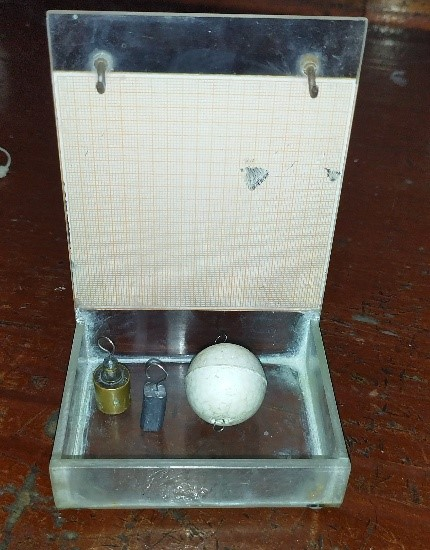
\includegraphics[width=0.8\linewidth,height=0.6\linewidth]{resources/mat2.jpg}
            \caption{Masas}
            \label{fig:mat2}
        \end{subfigure}
        \\
        \begin{subfigure}{0.5\textwidth} 
            \centering
            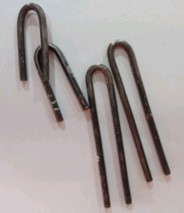
\includegraphics[width=0.8\linewidth,height=0.6\linewidth]{resources/mat3.jpg}
            \caption{Jinetillos}
            \label{fig:mat3}
        \end{subfigure}
        &
        \begin{subfigure}{0.5\textwidth} 
            \centering
            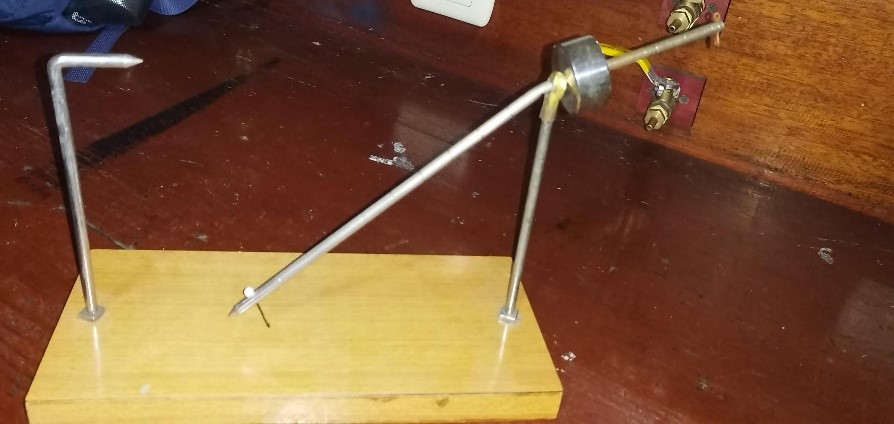
\includegraphics[width=0.8\linewidth,height=0.6\linewidth]{resources/mat4.jpg}
            \caption{Balanza de brazas}
            \label{fig:mat4}
        \end{subfigure}
        \\       
        \begin{subfigure}{0.5\textwidth} 
            \centering
            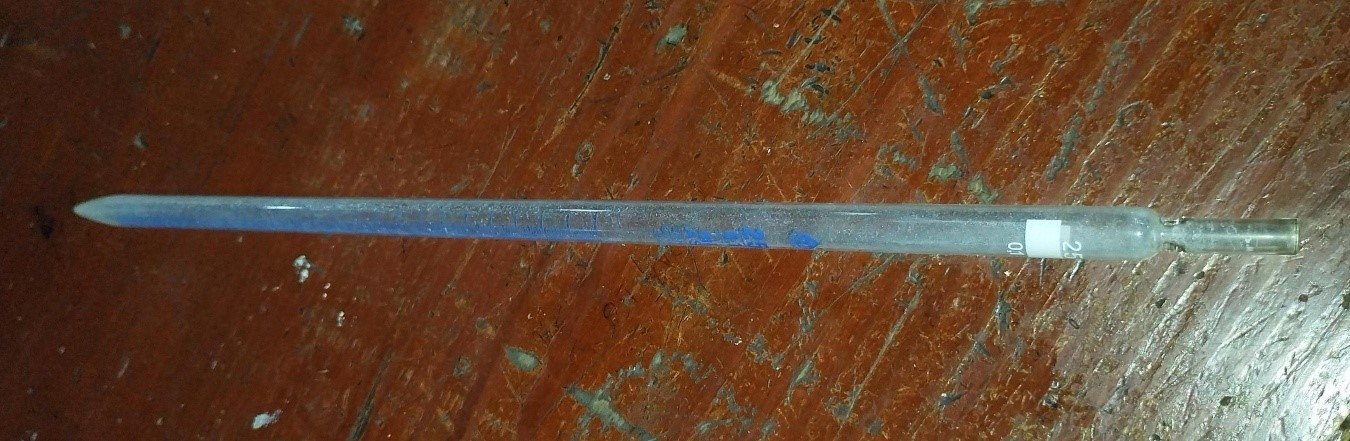
\includegraphics[width=0.8\linewidth,height=0.6\linewidth]{resources/mat5.jpg}
            \caption{Pipeta}
            \label{fig:mat5}
        \end{subfigure}
        &
        \begin{subfigure}{0.5\textwidth} 
            \centering
            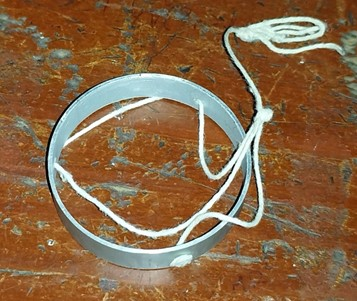
\includegraphics[width=0.8\linewidth,height=0.6\linewidth]{resources/mat6.jpg}
            \caption{Soporte}
            \label{fig:mat6}
        \end{subfigure}
        \\
    \end{tabular}
\end{figure}

\end{document}
